\documentclass{article}
\usepackage{tikz}
\usepackage[utf8]{inputenc}
\usepackage{ amssymb }
\usepackage{amsfonts}
\usetikzlibrary{automata,positioning,arrows}

\title{Autómatas y lenguajes formales. Tarea 2}
\author{Fabián Romero Jiménez}
\begin{document}
\maketitle
\begin{enumerate}
\item[\bf{Problema 1}] Minimiza el autómata de tu respuesta a los ejercicios 3 y 5 de la tarea 1.

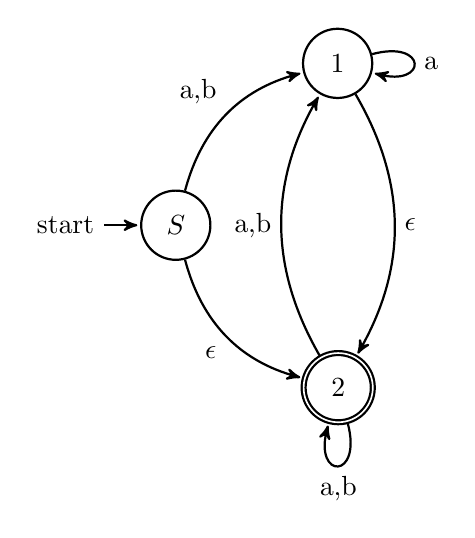
\begin{tikzpicture}[->,>=stealth',shorten >=1pt,auto,node distance=2cm,
  thick,main node/.style={circle,fill=blue!20,draw,font=\sffamily\Large\bfseries}]
   \node[state,initial] (q_0)   {$S$}; 
   \node[state] (q_1) [above right=of q_0] {$1$}; 
   \node[state,accepting] (q_2) [below right=of q_0] {$2$};
    \path[->] 
    (q_0) edge  [bend left] node {a,b} (q_1)
          edge  [bend right] node [swap] {$\epsilon$} (q_2)
    (q_1) edge  [bend left] node  {$\epsilon$} (q_2)
          edge [loop right] node {a} ()
    (q_2) edge  [bend left] node  {a,b} (q_1)
          edge [loop below] node {a,b} ();
\end{tikzpicture}
Transfórmalo en un autómata determinista usando los métodos vistos en clase. Minimiza el
resultado.\\


\item[Respuesta]

\begin{tabular}{ | l || l | l | l  |}
  \hline
    &  $a$    &   $b$  & $\epsilon^\star$ \\
  \hline
$>S$  &  1    &   1  &  S,2 \\    
1   &  1    &   -  &  1,2 \\
(2) &  2    &   2  &  2 \\
  \hline  
\end{tabular}

\begin{tabular}{ | l | l | l |}
  \hline
    &  $a\epsilon^\star$    &   $b\epsilon^\star$  \\
  \hline
$>S$   &  1,2 &   1,2 \\ 
$(1,2)$  &  1,2 &   1,2 \\ 
  \hline  
\end{tabular}


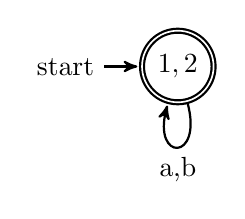
\begin{tikzpicture}[->,>=stealth',shorten >=1pt,auto,node distance=2cm,
  thick,main node/.style={circle,fill=blue!20,draw,font=\sffamily\Large\bfseries}]
   \node[state,initial,accepting] (q_0)   {$1,2$}; 
    \path[->] 
    (q_0) edge [loop below] node {a,b} ();
\end{tikzpicture}

\item[\bf{Problema 5}]Construye un autómata que acepte el lenguaje generado por la expresión $(0+1(01^\star 0)^\star 1)^\star $.
Aplica el algoritmo de minimalización a tu autómata.

Entonces, tenemos los simbolos $010101$ por lo que empezamos poniendo los 6 estados $q_0,q_1,..,q_5$ que corresponen a los símbolos en la expresión y el estado inicial $S$, además por cada simbolo + hacemos una bifurcación y por cada $\star$ una transición $\epsilon$ a donde empieza, así tenemos inicialmente el NFA

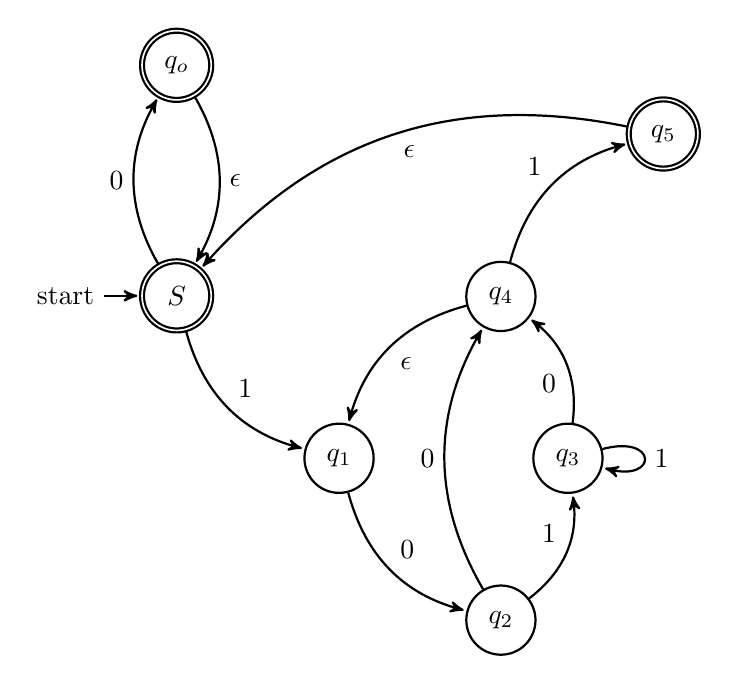
\begin{tikzpicture}[->,>=stealth',shorten >=1pt,auto,node distance=2cm,
  thick,main node/.style={circle,fill=blue!20,draw,font=\sffamily\Large\bfseries}]
   \node[state,initial,accepting] (S)   {$S$};
   \node[state,accepting]         (q_0)  [above=of S]   {$q_o$};
   \node[state ]                  (q_1)  [below right=of S]   {$q_1$};
   \node[state ]                  (q_2)  [below right=of q_1] {$q_2$};
   \node[state ]                  (q_3)  [right=of q_1]       {$q_3$};
   \node[state ]                  (q_4)  [above right=of q_1]   {$q_4$};
   \node[state,accepting]         (q_5)  [above right=of q_4]   {$q_5$};
   \path[->] 
    (S)   edge    [bend left]   node        {0}           (q_0)
          edge    [bend right]  node        {1}           (q_1)
    (q_0) edge    [bend left]   node        {$\epsilon$}  (S)
    (q_1) edge    [bend right]   node       {0}           (q_2)
    (q_2) edge    [bend right]   node       {1}           (q_3)
          edge    [bend left]   node        {0}           (q_4)
    (q_3) edge    [bend right]   node        {0}           (q_4)
          edge    [loop right]   node        {1}           ()
    (q_4) edge    [bend left]   node        {1}           (q_5)
          edge    [bend right]   node        {$\epsilon$}  (q_1)
    (q_5) edge    [bend right]  node         {$\epsilon$}  (S);
\end{tikzpicture}

Y lo transformamos en un DFA

\begin{tabular}{ | l || l | l | l  |}
  \hline
    &  $0$    &   $1$  & $\epsilon^\star$ \\
  \hline
$(>S)$  &  $q_0$   &   $q_1$  &  $S$       \\    
$(q_0)$ &  --      &   -      &  $S,q_0$   \\
$q_1$   &  $q_2$   &   -      &  $q_1$     \\
$q_2$   &  $q_4$   &   $q_3$  &  $q_2$     \\
$q_3$   &  $q_4$   &   $q_3$  &  $q_3$     \\
$q_4$   &  --      &   $q_5$  &  $q_4,q_1$ \\
$(q_5)$ &  --      &   -      &  $q_5,S$   \\
  \hline  
\end{tabular}

\begin{tabular}{ | l || l | l | l  |}
  \hline
    &  $0\epsilon^\star$    &   $1\epsilon^\star$  \\
  \hline
$(>S)$   &   $S,q_0$  &  $q_1$   \\    
$(S,q_0)$&   $S,q_0$  &  $q_1$   \\
$q_1$    &   $q_2$    &  --      \\
$q_2$    &   $q_4,q_1$&  $q_3$   \\
$q_4,q_1$&   $q_2$    &  $q_5,S$ \\
$q_3$    &   $q_4,q_1$&  $q_3$   \\
$(q_5,S)$&   $q_0,S$  &  $q_1$   \\
  \hline  
\end{tabular}

Así tenemos el DFA

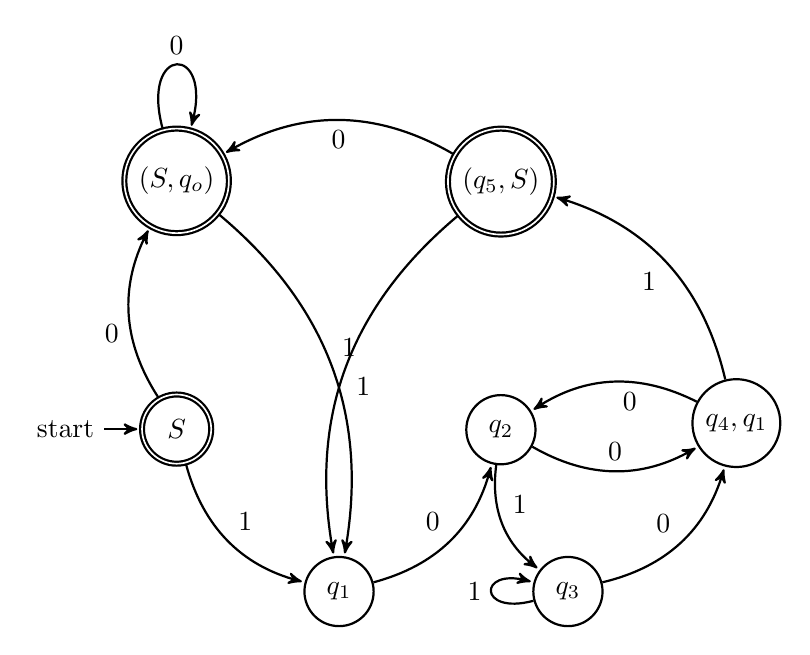
\begin{tikzpicture}[->,>=stealth',shorten >=1pt,auto,node distance=2cm,
  thick,main node/.style={circle,fill=blue!20,draw,font=\sffamily\Large\bfseries}]
   \node[state,initial,accepting] (S)   {$S$};
   \node[state,accepting]         (q_0)  [above=of S]           {$(S,q_o)$};
   \node[state ]                  (q_1)  [below right=of S]     {$q_1$};
   \node[state ]                  (q_2)  [above right=of q_1]   {$q_2$};
   \node[state ]                  (q_3)  [right=of q_1]         {$q_3$};
   \node[state ]                  (q_4)  [above right=of q_3]   {$q_4,q_1$};
   \node[state,accepting]         (q_5)  [above=of q_2]   {$(q_5,S)$};
    \path[->] 
    (S)   edge    [bend left]   node        {0}           (q_0)
          edge    [bend right]  node        {1}           (q_1)
    (q_0) edge    [loop above]   node        {0}           (q_0)
          edge    [bend left]   node        {1}           (q_1)
    (q_1) edge    [bend right]   node       {0}           (q_2)
    (q_2) edge    [bend right]   node       {0}           (q_4)
          edge    [bend right]   node        {1}           (q_3)
    (q_4) edge    [bend right]   node        {0}           (q_2)
          edge    [bend right]   node        {1}           (q_5)
    (q_3) edge    [bend right]   node        {0}           (q_4)
          edge    [loop left]   node        {1}          ()
    (q_5) edge    [bend right]  node         {0}          (q_0)
          edge    [bend right]  node         {1}          (q_1);
\end{tikzpicture}

Minimizando tenemos:
$$ \{q_1,q_2,q_3,(q_4,q_1)\} , \{S,(q_0,s),(q_5,S)\} $$
\\Separando $(q_4,q_1)$  pues con entrada $1$ va a un estado final
$$ \{q_2,q_3\}, \{(q_4,q_1),q1\} , \{S,(q_0,s),(q_5,S)\} $$

y finalmente tenemos el DFA minimizado:

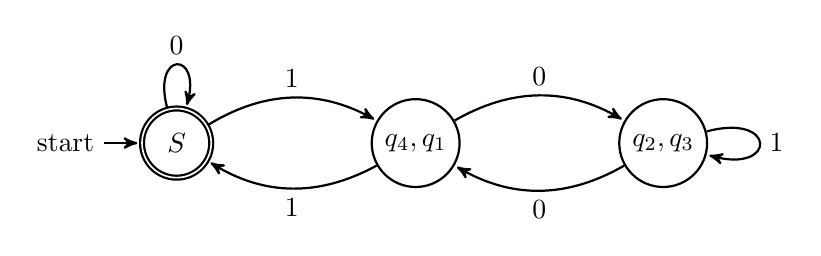
\begin{tikzpicture}[->,>=stealth',shorten >=1pt,auto,node distance=2cm,
  thick,main node/.style={circle,fill=blue!20,draw,font=\sffamily\Large\bfseries}]
   \node[state,initial,accepting] (S)   {$S$};
   \node[state ]                  (q_4)  [right=of S]           {$q_4,q_1$};
   \node[state ]                  (q_2)  [right=of q_4]        {$q_2,q_3$};
    \path[->] 
    (S)   edge    [loop above]   node        {0}          ()
          edge    [bend left]  node        {1}          (q_4)
    (q_2) edge    [bend left]   node       {0}          (q_4)
          edge    [loop right]   node        {1}          ()
    (q_4) edge    [bend left]   node        {0}         (q_2)
          edge    [bend left]   node        {1}         (S);
\end{tikzpicture}


\item[\bf{Problema 2}].  Considera el siguiente sistema de ecuaciones


$ X_0 = a \cdot (X_1 \wedge X_2) + b \cdot X_o +0 $\\
$ X_1 = b \cdot (\bar{X_0} \vee X_2) + a \cdot X_o + \epsilon $\\
$ X_2 = a \cdot (X_1 \vee \bar{X_2}) + b \cdot (\bar{X_1} \wedge X_2) + \epsilon$

Lo que nos indica que hay 3 estados, $s$ que es testado inicial
y $(1)$ y $(2)$ que son de aceptación, debido a que sus ecuaciones $X_1$ y $X_2$ tienen constante $\epsilon$, como la ecuación de $s$ tiene como conastante $0$, no es un estado de aceptación, y la tabla de transiciones es la siguiente:

\begin{tabular}{ | l || l | l | l  |}
  \hline
Estado    &  a    &   b  \\
  \hline
$>s$   &   $1 \wedge 2$  &  $ s $   \\    
$(1)$  &   $ s $  &  $ 2  \vee \neg s$   \\
$(2)$  &   $ 1 \vee \neg 2$    &  $\neg 1 \wedge 2 $ \\
  \hline  
\end{tabular}


\item[\bf{Problema 3}]. Construye el autómata de diccionario para el conjunto $X = \{ab, ba, aba, bab\}$ con el alfabeto $\Sigma = \{a, b, c\}$.


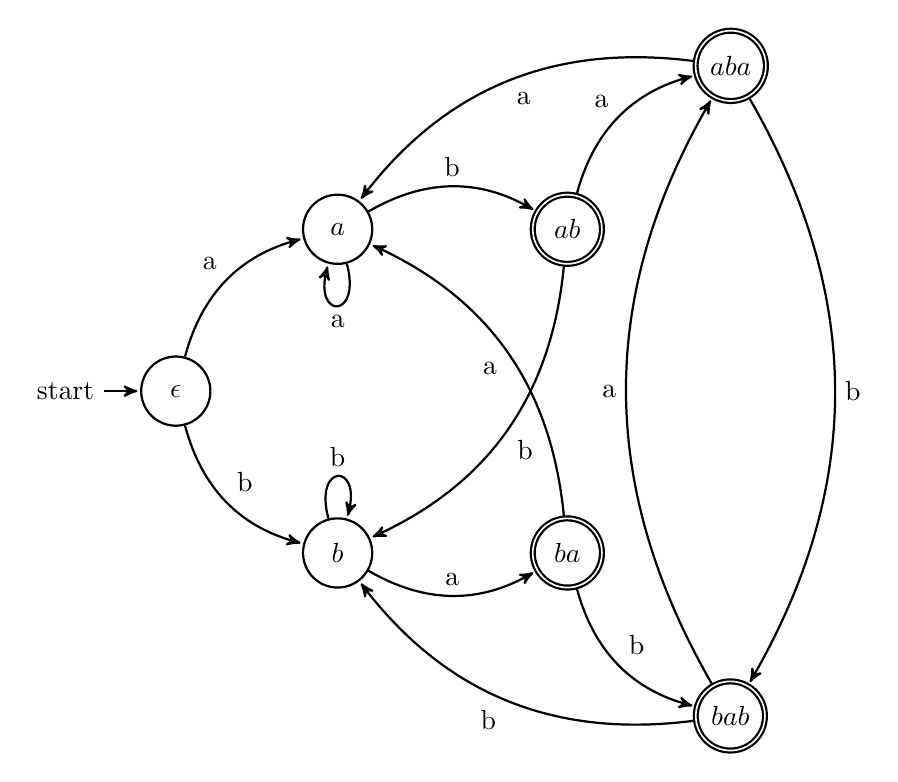
\begin{tikzpicture}[->,>=stealth',shorten >=1pt,auto,node distance=2cm,
  thick,main node/.style={circle,fill=blue!20,draw,font=\sffamily\Large\bfseries}]
   \node[state,initial]    (S)   {$\epsilon$};
   \node[state ]           (a)   [above right=of S] {$a$};
   \node[state,accepting ] (ab)  [right=of a] {$ab$};
   \node[state,accepting ] (aba) [above right=of ab] {$aba$};
   \node[state ]           (b)   [below right=of S] {$b$};
   \node[state,accepting ] (ba)  [right=of b] {$ba$};
   \node[state,accepting ] (bab) [below right=of ba] {$bab$};
   \path[->] 
    (S)   edge    [bend left]   node        {a}           (a)
          edge    [bend right]  node        {b}           (b)
    (a)   edge    [loop below]  node        {a}           ()
          edge    [bend left]  node        {b}           (ab)
    (b)   edge    [loop above]  node        {b}           ()
          edge    [bend right]  node        {a}           (ba)
    (ab)  edge    [bend left]  node        {a}           (aba)
          edge    [bend left]  node         {b}           (b)
    (ba)  edge    [bend right]  node        {b}           (bab)
          edge    [bend right]  node         {a}           (a)
    (aba) edge    [bend right]  node         {a}           (a)
          edge    [bend left]  node         {b}           (bab)
    (bab) edge    [bend left]  node         {a}           (aba)
          edge    [bend left]  node         {b}           (b);
\end{tikzpicture}


\item[\bf{Problema 4}].
Considera la siguiente descripción de un lenguaje de programación simple:
\begin{itemize}
\item Localidades de memoria: $X, Y, Z, X_1 , . . .$;
\item Constantes: $0, 1, -1, ...$;
\item Expresiones aritméticas: (a) localidades; (b) constantes; (c) si a y b son expresiones
aritméticas, también lo son ($a + b$), ($a \times b$) y ($a-b$);
\item Constantes boolenas: V y F;
\item Comparaciones: ($X = a$) y ($X < a$), donde X es una localidad y a una expresión
aritmética;
\item Expresiones booleanas: (a) constantes booleanas; (b) comparaciones; (c) si b y v son
expresiones booleanas, también lo son $\neg b$, ($b \vee v$) y ($b \wedge v$);
\item Asignaciones: $X := a$, donde $X$ es una localidad y a una expresión aritmética;
\item El programa $skip$;
\item Programas: (a) skip; (b) asignaciones; (c) si P y Q son programas y b es una expresión booleana, los siguientes también son programas: (P; Q), (if b then P else Q) y (while b do P).
\end{itemize}

\item[\bf{CFG}] 

$P \rightarrow skip |N|$ if $B$ then $P$ else $P |$ while $B$ do $P$   // Programa\\ 
$N \rightarrow A|E|N;N$ // Predicado\\
$B \rightarrow v|f|E<E|E=E|\neg B |B \vee B| B \wedge B $ // Expresión Booleana\\
$A \rightarrow L:=E$ // Asignación\\
$E \rightarrow C|-C|E+E|E-E|E \times E$ //Expresión\\
$L \rightarrow x|y|z|LC$ // Localidad\\
$C \rightarrow 0|1|2|..|9|CC$ // Constante


\item[\bf{Problema 5}] Da gramáticas en forma normal de Chomsky y de Greibach del mismo lenguaje

\item[\bf{CNF}]
$ IF    \rightarrow if$\\
$ THEN  \rightarrow then$\\
$ ELSE  \rightarrow else$\\
$ W \rightarrow while$\\
$ DO    \rightarrow do$\\
$ A_{:=}    \rightarrow  := $\\
$ N_{;}     \rightarrow  ; $\\
$ E_{+}     \rightarrow  + $\\
$ E_{\times} \rightarrow  \times $\\
$ E_{-}     \rightarrow  - $\\
$ B_{<} \rightarrow < $\\
$ B_{=} \rightarrow = $\\
$ B_{\neg} \rightarrow \neg $\\
$ B_{\vee} \rightarrow \vee $\\
$ B_{\wedge} \rightarrow \wedge $\\
$ L        \rightarrow  x|y|z|L$ $C  $\\
$ C     \rightarrow  0|1|2|3|4|5|6|7|8|9|CC$\\

$P_{0} \rightarrow skip |L$ $N_{asign_1}|E$ $E_{+1}|E$ $E_{\times1}|E$ $E_{-1}|E_{-}$ $C|N N_{sep_1}| IF$ $P_{if_1} |W$ $P_{w_1}$\\
$P \rightarrow skip |L$ $N_{asign_1}|E$ $E_{+1}|E$ $E_{\times1}|E$ $E_{-1}|E_{-}$ $C|N N_{sep_1}| IF$ $P_{if_1} |W$ $P_{w_1}$\\
$P_{if_1} \rightarrow B$ $P_{if_2}$\\
$P_{if_2} \rightarrow THEN$ $P_{if_3}$\\
$P_{if_3} \rightarrow P$ $P_{if_4}$\\
$P_{if_4} \rightarrow ELSE$ $P$\\
$P_{w_1} \rightarrow B$ $P_{w_2}$\\
$P_{w_2} \rightarrow DO$ $P$\\
$N_{sep_1}  \rightarrow N_{;}$ $N$\\
$N_{asign_1} \rightarrow A_{:=}$ $N$\\
$B \rightarrow v|f| E$ $B_{<1} | E$ $B_{=1} | B$ $B_{\wedge 1} | B$  $B_{\vee 1} | B_{\neg}$ $B $\\
$B_{=1} \rightarrow B_{=}$ $E$\\
$B_{<1} \rightarrow B_{<}$ $E$\\
$E \rightarrow 0|1|2|3|4|5|6|7|8|9|E$ $E|E_{-} E|E$ $E_{+1}|E$ $E_{-1}|E$ $E_{\times1}$\\
$E_{+1} \rightarrow E_{+}$ $E$\\
$E_{-1} \rightarrow E_{-}$ $E$\\
$E_{\times1} \rightarrow E_{\times}$ $E$\\


\item[\bf{GNF}]

$P \rightarrow skip |N|$ if $B$ then $P$ else $P |$ while $B$ do $P$   // Programa\\ 
$N \rightarrow A|E|N;N$ // Predicado\\
$B \rightarrow v|f|E<E|E=E|\neg B |B \vee B| B \wedge B $ // Expresión Booleana\\
$A \rightarrow L:=E$ // Asignación\\
$E \rightarrow C|-C|E+E|E-E|E \times E$ //Expresión\\
$L \rightarrow x|y|z|LC$ // Localidad\\
$C \rightarrow 0|1|2|..|9|CC$ // Constante




\item[\bf{Problema 6}]  Describe un NPDA que acepte este lenguaje de programación.

En general, podemos convertir cualquier CFG dado en  GNF a un NPDA de la siguiente forma:\\

sea $G=(\Sigma_g,\Gamma_g,S_g,\rightarrow_g)$ la Gramática en GNF, 
costruimos una NPDA $M=(Q_m,\Sigma_m,\Gamma_m, \gamma_m,s_m)$ con aceptación con pila vacía siguiendo las reglas:\\
$Q_m={q}$ Un único estado\\
$\Sigma_m = \Gamma_g$ Los símbolos de entrada de M, son los simbolos terminales de $G$
$\Gamma_m = \Sigma_g$ Los símbolos de pila de M, son todos los simbolos de de $G$
$s_m = S_g$ El simbolo inicial de M es el simbolo inicial de G.

Las función de transición será la siguiente:\\
para toda $\alpha \in \Sigma_g$ es decir, para todos los simbolos terminales, hay una transición:\\
$\delta(q,a,a)=(q,\epsilon)$
como esta en GNF, las otras producciones del tipo $$\beta \rightarrow \alpha\beta_1\beta_2...\beta_n$$
se agrega a la función de transición:
$\delta(q,\alpha,\beta) = (q,\beta_1\beta_2...\beta_n)$
en caso de que sea n sea 0 es decir una producción de la forma $\beta \rightarrow \alpha$  se agrega $\delta(q,\alpha,\beta) = (q,\epsilon)$

y este NPDA acepta el mismo lenguage que la CFG en GNF dada.

\item[\bf{Problema 7}]  El teorema de Chomsky-Schützenberger nos dice que hay existen $n \in \mathbb{N}, R \in Reg$ tales que existe un homomorfismo entre $D^{\star}_n \cap R$ y el lenguaje de programación anterior. Da un valor de n y justifica tu respuesta.

\item[\bf{Respuesta}]
El teorema de Chomsky-Schützenberger nos muestra en su construcción que si un lenguaje libre de contexto esta dado en CNF se puede hacer un isomormismo ente cada simbolo terminal a un tipo de parentesis, y cada producción a no terminales a 2 pares, asi, en el CNF dado aqui, tiene 28 producciones a simbolos terminales y 33 producciones a no terminales, por lo que 94 tipos de caracteres son suficientes para este lenguage

\item[\bf{Problema 8}]  Da CFG para los lenguages:

\item[\bf{a)}]  $ \{a^{n}b^{2n}c^{k}| 1 \le k,n \}$\\
$S \rightarrow Ac|Sc $\\
$A \rightarrow aAbb|abb $

\item[\bf{b)}]  $ \{a^{k}b^{m}c^{n}| 1 \le k,m,n, n\le 2k\}$\\

$S \rightarrow aaAc|aaSc $\\
$A \rightarrow aA|Ab|b $\\

\item[\bf{c)}]  $ \{a,b\}^{\star} - \{palindromas\}$\\

$S \rightarrow aSa| bSb | aSb | bSa | AB | BA $\\
$A \rightarrow a|aA $\\
$B \rightarrow b|bB $\\

\item[\bf{Problema 9}] Demuestra que los siguientes conjuntos no son CFL:
\item[\bf{a)}]  $\{a^{n}b^{m}c^{k}d^{n}| 2n=3m \wedge 5k=7m  \}$\\
si $2n=3m$ y $5k=7m$ tenemos que $2|m$ y $5|m$ asi que $10|m$ por lo que diremos que $m=10m'$
como $2n=3m$ tenemos que $2n=30m'$ y entonces $n=15m'$, análogamente por $5k=7m$ tenemos que $5k=70m'$ y $k=14m'$
así el lenguage lo podemos expresar como $\{a^{15m'}b^{10m'}c^{14m'}d^{15m'}| m \in \mathbb{N}  \}$\\
como a aparece siempre en potencias de 15, sea $a_1=a^{15}$ y análogamente $b_1=b^{10}$,$c_1=b^{14}$ y $d_1=d^{15}$
por lo que tenemos que encontrar si el lenguage descrito como $\{a_1^{m'}b_1^{m'}c_1^{m'}d_1^{m'}\}$ es un CFL.
pero por el lema del bombeo sea $m'>k$ donde $k$ es la constante para el CFL.\\
donde tenemos que $z= a_1^{m'}b_1^{m'}c_1^{m'}d_1^{m'} = \beta \gamma \eta \theta \psi $ donde $ \gamma \theta \ne \epsilon$ y $|\gamma \eta \theta | \le k$
así $\gamma \eta \theta$ puede contener cuando más dos tipos diferentes de simbolos $a_1,b_1,c_1,d_1$ pues cada simbolo se repite $k$ veces consecutivas.
por lo que $\gamma^i \eta \theta^i$ inserta al menos un tipo de simbolo y cuando más dos, pero el lenguage requiere que los cuatro simbolos se agregen en las mismas
cantidades, por lo que el lenguage no es CFG $\blacksquare$

\item[\bf{b)}]  $ \{a^{i}b^{j}c^{k}d^{l} | i=k, j=l \}$\\
elijamos $i,j > k$ donde $k$ es la constante para el CFL.\\
tenemos que $z= a^{i}b^{j}c^{i}d^{j} = \beta \gamma \eta \theta \psi $ donde $ \gamma \theta \ne \epsilon$ y $|\gamma \eta \theta | \le k$
así $\gamma \eta \theta$ puede contener cuando más dos tipos diferentes de simbolos $a,b,c,d$ pues cada simbolo se repite más de $k$ veces consecutivas.
por lo que $\gamma^i \eta \theta^i$ inserta al menos un tipo de simbolo y cuando más dos, pero el lenguage requiere que los cuatro simbolos se agregen por pares en las mismas
cantidades, por lo que el lenguage no es CFG $\blacksquare$



\item[\bf{Problema 10}] Describe detalladamente la ejecución del algoritmo CKY para decidir si la cadena $((x = 0) \vee f)$ es una expresión booleana:


Primero el subconjunto requerido de la grámatica de evaluación booleana en CNF.

$S  \rightarrow  P_a$ $S_c | S$ $S_{\vee1} | V$ $E_{=1} |v|f$\\
$P_a \rightarrow ( $\\
$P_c \rightarrow$ $) $\\
$S_= \rightarrow$ $= $\\
$E_+ \rightarrow$ $+ $\\
$S_c \rightarrow  S$ $P_{c} $\\
$S_{\vee1} \rightarrow  S_{\vee}$ $S $\\
$E_{=1} \rightarrow  S_=$ $S $\\
$E \rightarrow 0|1|2|..|9|E$ $E_{+1} $\\
$E_{+1} \rightarrow E_+$ $E$\\
$V \rightarrow x|y|z $\\

En este caso, como esta puesta con parentesis elimina rápidamente las opciones.
Así

\begin{tabular}{ |l|l|l|l|l|l|l|l|l||l|}
  \hline
 ( & ( & x & = & 0 & ) & $\vee$ & f & ) & Cadena Reconocida \\
\hline  
$P_a$ & $P_a$ & $V$ & $S_=$ & $E$ & $P_c$ & $S_{\vee}$ & $S$ & $P_C$ &\\
 - & - & - & - & - & - & -  & - & &\\
 - & - & $S$ & - & - & - & -  & - & & $x=0$\\
 - & $S$ & - & - & - & - & - &  & & $(x=0$\\
 - & $S$  & - & - & - & - &  &  & & $(x=0)$\\
 - & -  & - & - & - &  &  &  & & \\
 - & $S$ & - & - &  &  &  &  & &  $(x=0) \vee f$ \\
 $S$ & - &  &  &  &  &  &  & &  $((x=0) \vee f$ \\
 $S$ &  &  &  &  &  &  &  & &  $((x=0) \vee f)$ \\
\hline  
\end{tabular}\\
Solo tiene una producción que genera la cadena deseada y empieza en $S$, por lo que la parsea de forma no ambigua

\end{enumerate}



\end{document}  
